% Intended LaTeX compiler: pdflatex
\documentclass[10pt,a4paper,UTF8]{article}
\usepackage{zclorg}
\usepackage{tikztheorem}
\author{zcl.space}
\date{}
\title{负二项随机变量分布}
\hypersetup{
 pdfauthor={zcl.space},
 pdftitle={负二项随机变量分布},
 pdfkeywords={probability},
 pdfsubject={},
 pdfcreator={Emacs 25.0.50.1 (Org mode 9.0.6)},
 pdflang={English}}
\begin{document}

\maketitle
\tableofcontents
\titlepic{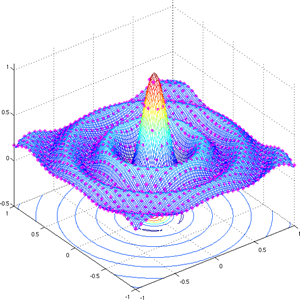
\includegraphics[scale=0.25]{../../img/sinc.PNG}}

\section{负二项随机变量}
\label{sec:orgd79b8cc}


假定独立重复试验中,每次成功的概率为\(p\),试验持续进行直到试验累积成功\(r\)次为止,如果我们令\(X\)表示试验的总次数,则:
\begin{equation}
\label{eq:1}
P\{X=n\} = \binom{n-1}{r-1} p^{r}(1-p)^{n-r}, \quad n= r,r+1,\ldots
\end{equation}

分析:直到\(r\)次成功,意味着前面\(n-1\)次成功了\(r-1\)次,概率为:\[\binom{n-1}{r-1}p^{r-1}(1-p)^{n-r}\]最后一次成功的概率为\(p\),所以式 (\ref{eq:1})成立。

我们接下来要证明一件事情:试验一直持续下去肯定会有\(r\)次成功,即:
\begin{equation}
\label{eq:2}
\sum_{n=r}^{\infty}P\{X=n\} = \sum_{n=r}^{\infry} \binom{n-1}{r-1}p^{r}(1-p)^{n-r} = 1
\end{equation}
上式可以从分析的角度来证明,当然我们不会这么傻,我们希望从概率的角度来证明,我们要赋予上式数学意义。考虑获得\(r\)次成功所需要的实验次数可以分解为\(Y_{1} +Y_{2} + \ldots + Y_{r}\),其中\(Y_{1}\)表示第1次成功需要的实验次数,\(Y_{2}\)表示从第一次到第二次成功用的试验次数,\(Y_{r}\)表示从第\(r-1\)到第\(r\)次成功需要的实验次数。因为试验是相互独立的所以\(Y_{1},\ldots ,Y_{r}\)都是几何随机变量。而几何随机变量都是以概率1取有限值,也就是说对于几何随机变量来说总会成功的,对于负二项随机变量来说成功一次就肯定可以成功\(r\)次。
\section{负二项随机变量的期望和方差}
\label{sec:orga924efc}


我们有:
\begin{eqnarray}
\label{eq:3}
E[X^{k}] &=& \sum_{n=r}^{\infty}n^{k}\binom{n-1}{r-1}p^{r}(1-p)^{n-r}\\
&=& \frac{r}{p}\sum_{n=r}^{\infty} n^{k-1}\binom{n}{r}p^{r+1}(1-p)^{n-r} \\
&=& \frac{r}{p} \sum_{n=r+1}^{\infty} (m-1)^{k-1} \binom{m-1}{r}p^{r+1}(1-p)^{m-(r+1)} \\
&=&\frac{r}{p}E[(Y-1)^{k-1}]
\end{eqnarray}

其中\(Y\)是参数为\((r+1,p)\)的负二项随机变量。在上式中令\(k=1\),则:
\begin{equation}
\label{eq:4}
E[X] = \frac{r}{p}
\end{equation}
令\(E[X^{k}]\)中\(k=2\),并利用负二项随机变量的期望公式有:
\begin{equation}
\label{eq:5}
E[X^{2}] = \frac{r}{p}E[Y-1] = \frac{r}{p}(\frac{r+1}{p} - 1)
\end{equation}

因此:
\begin{equation}
\label{eq:6}
\mathrm{Var}(X) = \frac{r}{p}( \frac{r+1}{p} -1) - (\frac{r}{p})^{2}
\end{equation}
在独立重复试验中,如果每次试验成功的概率为\(p\),则累积\(r\)次成功的总试验次数的期望和方差分别为\(r/p\)和\(r(1-p)/p^{2}\)。注意这个结果和 \href{geometry-distribution.org}{几何随机变量} 一文中的期望和方差的关系。
\section{例子}
\label{sec:orge3abb80}


\begin{tikzproblem}
独立重复试验中,设每次试验成功的概率为\(p\),求第\(r\)次成功发生在\(m\)次失败之前的概率。
\end{tikzproblem}

\begin{tikzanswer}
分析这个问题,可知,\(r\)次成功的时刻一定要在\(r\)次试验之后和\(r+m-1\)之前,才能保证在\(m\)次失败之前出现第\(r\)次成功。所以有:
\begin{equation}
\label{eq:7}
\sum_{n=r}^{r+m-1}\binom{n-1}{r-1}p^{r}(1-p)^{n-r}
\end{equation}
\end{tikzanswer}

\begin{tikzproblem}
某个抽烟的数学家总是随身带着两盒火柴,一盒放在左边口袋一盒放在右边口袋。每次他需要火柴时,都是随机的从两个口袋中任取一盒,并取出其中一根。如果假设开始时两盒火柴都有\(N\)根火柴,那么在他第一次发现其中一个盒子已经空了的时候,另一盒中恰好有\(k\)根的概率有多大,\(k=0,1,\ldots ,N\)?
\end{tikzproblem}

\begin{tikzanswer}
设\(E\)表示时间“数学家第一次发现右边口袋里的火柴盒是空的而此时左边口袋里的火柴盒里有\(k\)根火柴”。这个事件发生当且仅当第\((N+1+N-k)\)次抽取火柴证号取中的是右边口袋,而且第\(N+1\)次取中右边口袋。这个分布是负二项分布,其中\(p=1/2, r=N+1, n=2N-k+1\),有:
\begin{equation}
\label{eq:8}
P(E) = \binom{2N-k}{N}(\frac{1}{2})^{2N-k+1}
\end{equation}
又因为事件"第一次发现左边口袋里的火柴盒是空的,而此时右边口袋里恰好还有\(k\)根火柴"与E是等概率的。所以我们所求的概率为:
\begin{equation}
\label{eq:9}
2P(E) = \binom{2N-k}{N}(\frac{1}{2})^{2N-k}
\end{equation}
\end{tikzanswer}
\end{document}
